\section{Background and Motivation}
\label{sec:bg}

\subsection{LLM post-training}
\label{sec:bg-post-training}

\begin{figure}[!t]
    %    \vspace{-2mm}
        \begin{minipage}{1\linewidth}
        % \hspace{-3mm}
        \centering    
        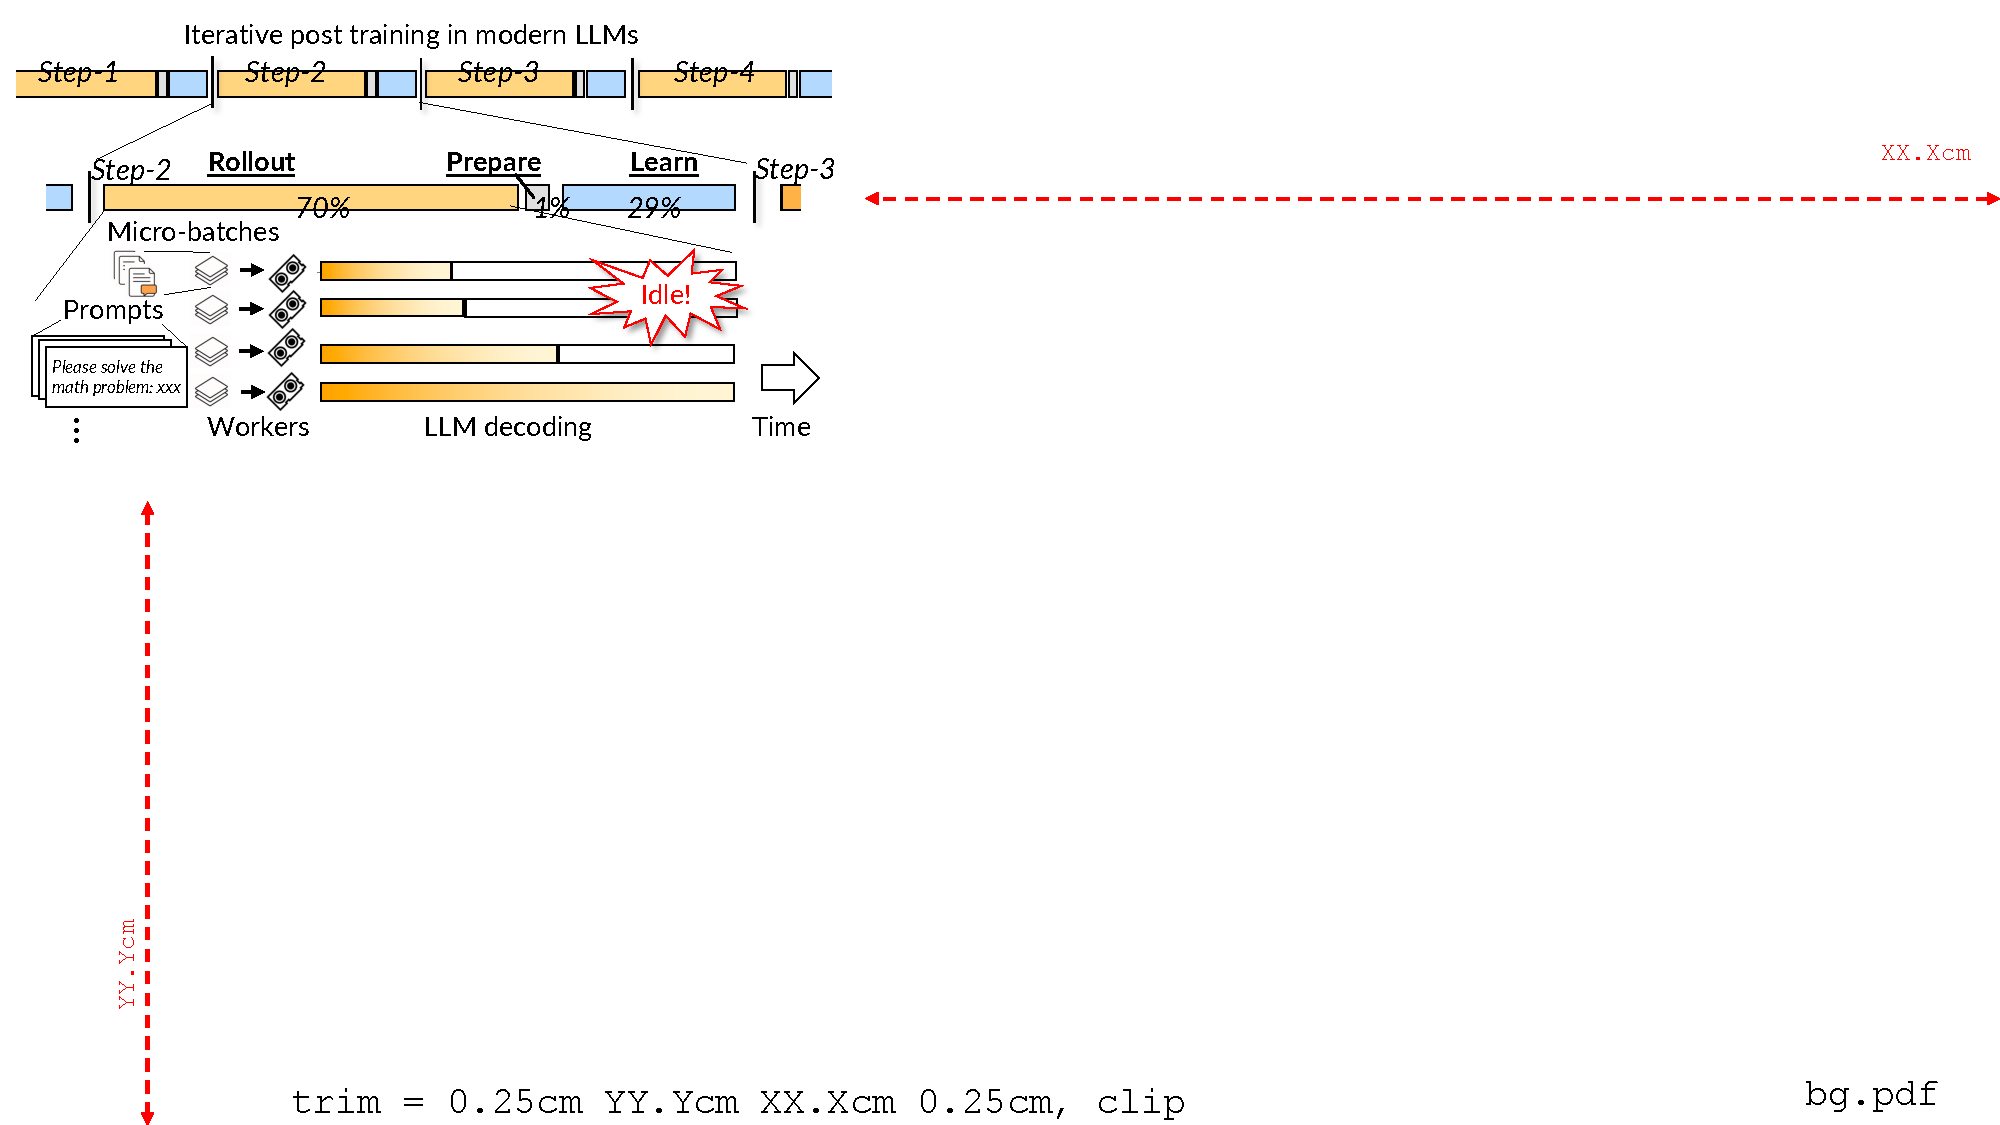
\includegraphics[width=1\linewidth, trim=0.25cm 10.95cm 19.4cm 0.25cm, clip]{figs/bg.pdf} 
        \end{minipage} \\[0pt]
        \begin{minipage}{1\linewidth}
        \caption{\small{%
            An illustration of the rollout process in LLM post-training. 
        }}
        \label{fig:bg-rollout}
        \end{minipage} \\[-20pt]
        \end{figure} 

\nospacestitle{Generation with LLM. \,}
Large Language Models (LLMs) generate responses (termed \emph{tokens}) through \emph{prefill} and \emph{decode} phases.
The prefill phase processes the initial input (termed \emph{prompt})
 to generate the first token.
The decode phase then iteratively generates subsequent tokens in an auto-regressive fashion
by combining previous output tokens with the original input as the new input.
The decode phase terminates upon generating an end-of-sequence token.

\stitle{Post-training workflow. \,}
Leading LLMs are post-trained with reinforcement learning (RL) 
with multiple steps of execution,
where each step follows an identical three phases~\cite{DBLP:journals/corr/abs-2501-12948,realhf,DBLP:conf/nsdi/ZhongZWLCWHXMZ025,hybridflow}: 

%\vspace{0.5ex}
\etitle{1. Rollout. \,}
% The training treats the model as RL actors and generates tokens
% from a sampled batch of pre-defined prompts using the aforementioned LLM generation process.
The process treats the trained model as actor and generates tokens
from a sampled batch of pre-defined prompts using LLM decoding.
The tokens are used to solve specific tasks like math problems. 
% To accelerate the rollout,
To accelerate rollout, the sampled batch is divided into smaller micro-batches 
(\emph{batch}\footnote{\footnotesize{Since we only refer to micro-batches in the following content,we use the more general term \emph{batch} to indicate micro-batch without loss of generality. }})
and processed concurrently 
by multiple rollout workers. 
Each worker deploys the model on one or more GPUs 
using model parallelism if necessary~\cite{hybridflow}.

Two aspects regarding rollout batch need to be noted.
% regarding the formulation of the rollout batch.
First, to improve efficiency, production RL training applies a relatively large
rollout batch size per step to find sufficient positive rewards~\cite{DBLP:conf/iclr/KeskarMNST17,DBLP:journals/corr/abs-2402-03300,DBLP:conf/nips/YaoGLKM18,dapo,gspo},
e.g., a typical 32B task
sets the per-step total batch size to {8\,K}~\cite{dapo,DBLP:journals/corr/abs-2504-05118}. 
% Second, each data point is typically seen a few times during the entire training process,
% \ie{most training involves only 1--2 epochs~\cite{deepseek-r1}},
% making n-gram-based techniques like 
% experience replay~\cite{liu2025specrlacceleratingonpolicyreinforcement} less effective.
Second, each prompt is typically seen only once or twice 
(\ie{common training involves just 1--2 epochs~\cite{deepseek-r1}}),
limiting the effectiveness of n-gram-based methods like experience replay
~\cite{liu2025specrlacceleratingonpolicyreinforcement,rhymerl}.


%\vspace{0.5ex}
\etitle{2. Prepare. \,} 
In the prepare phase, the rollout results are fed into
a set of judgers~\cite{DBLP:journals/corr/abs-2402-03300,dapo,DBLP:journals/corr/abs-2504-02605,DBLP:journals/corr/abs-2509-02547}
(e.g., a separate reward model)
to generate rewards~\cite{DBLP:journals/corr/SchulmanWDRK17,DBLP:journals/corr/abs-2204-05862},
which are the arithmetic signals that guide the parameter optimization.
These judgers are lightweight; for example, the reward models only compute a forward pass,
rather than auto-regressive generation,
so the time required is negligible in a training step.

%\vspace{0.5ex}
\etitle{3. Learn. \,}
Given the signals from the prepare phase, the learning phase 
calculates the loss and updates the LLM parameters
with a backward pass.
The updated parameters are then used in the next rollout step. 
%similar to pre-training~\cite{DBLP:conf/sosp/NarayananHPSDGG19,DBLP:journals/corr/abs-1909-08053}.
%% XD: don't know the meaning of the below sentence
%Due to memory limit, production training would split mini-batch
%into micro-batches and update gradient separately~\cite{dapo,DBLP:journals/corr/abs-2504-05118}.



\begin{figure}[!t]
    %    \vspace{2mm}
        \begin{minipage}{1\linewidth}
        \hspace{-1mm}
        \centering    
        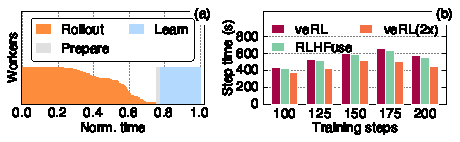
\includegraphics[width=\columnwidth]{data/motiv-rollout.pdf} \\[1pt]    
        \end{minipage} \\[0pt]
        \begin{minipage}{1\linewidth}
        \caption{\small{%
        {
            (a) {The long rollout in post-training}
            and (b) the training latency of various steps
            in DAPO-32B-20K training trace (detailed setups described in \textsection{\ref{sec:eval-setup}}). 
        }}}
        \label{fig:data-motivation}
        \end{minipage} \\[-5pt]
\end{figure}

\subsection{Analysis of post-training and current solutions}
\label{sec:bg-motivation}

\begin{figure}[!t]
    %    \vspace{-2mm}
        \begin{minipage}{1\linewidth}
        % \hspace{-3mm}
        \centering    
        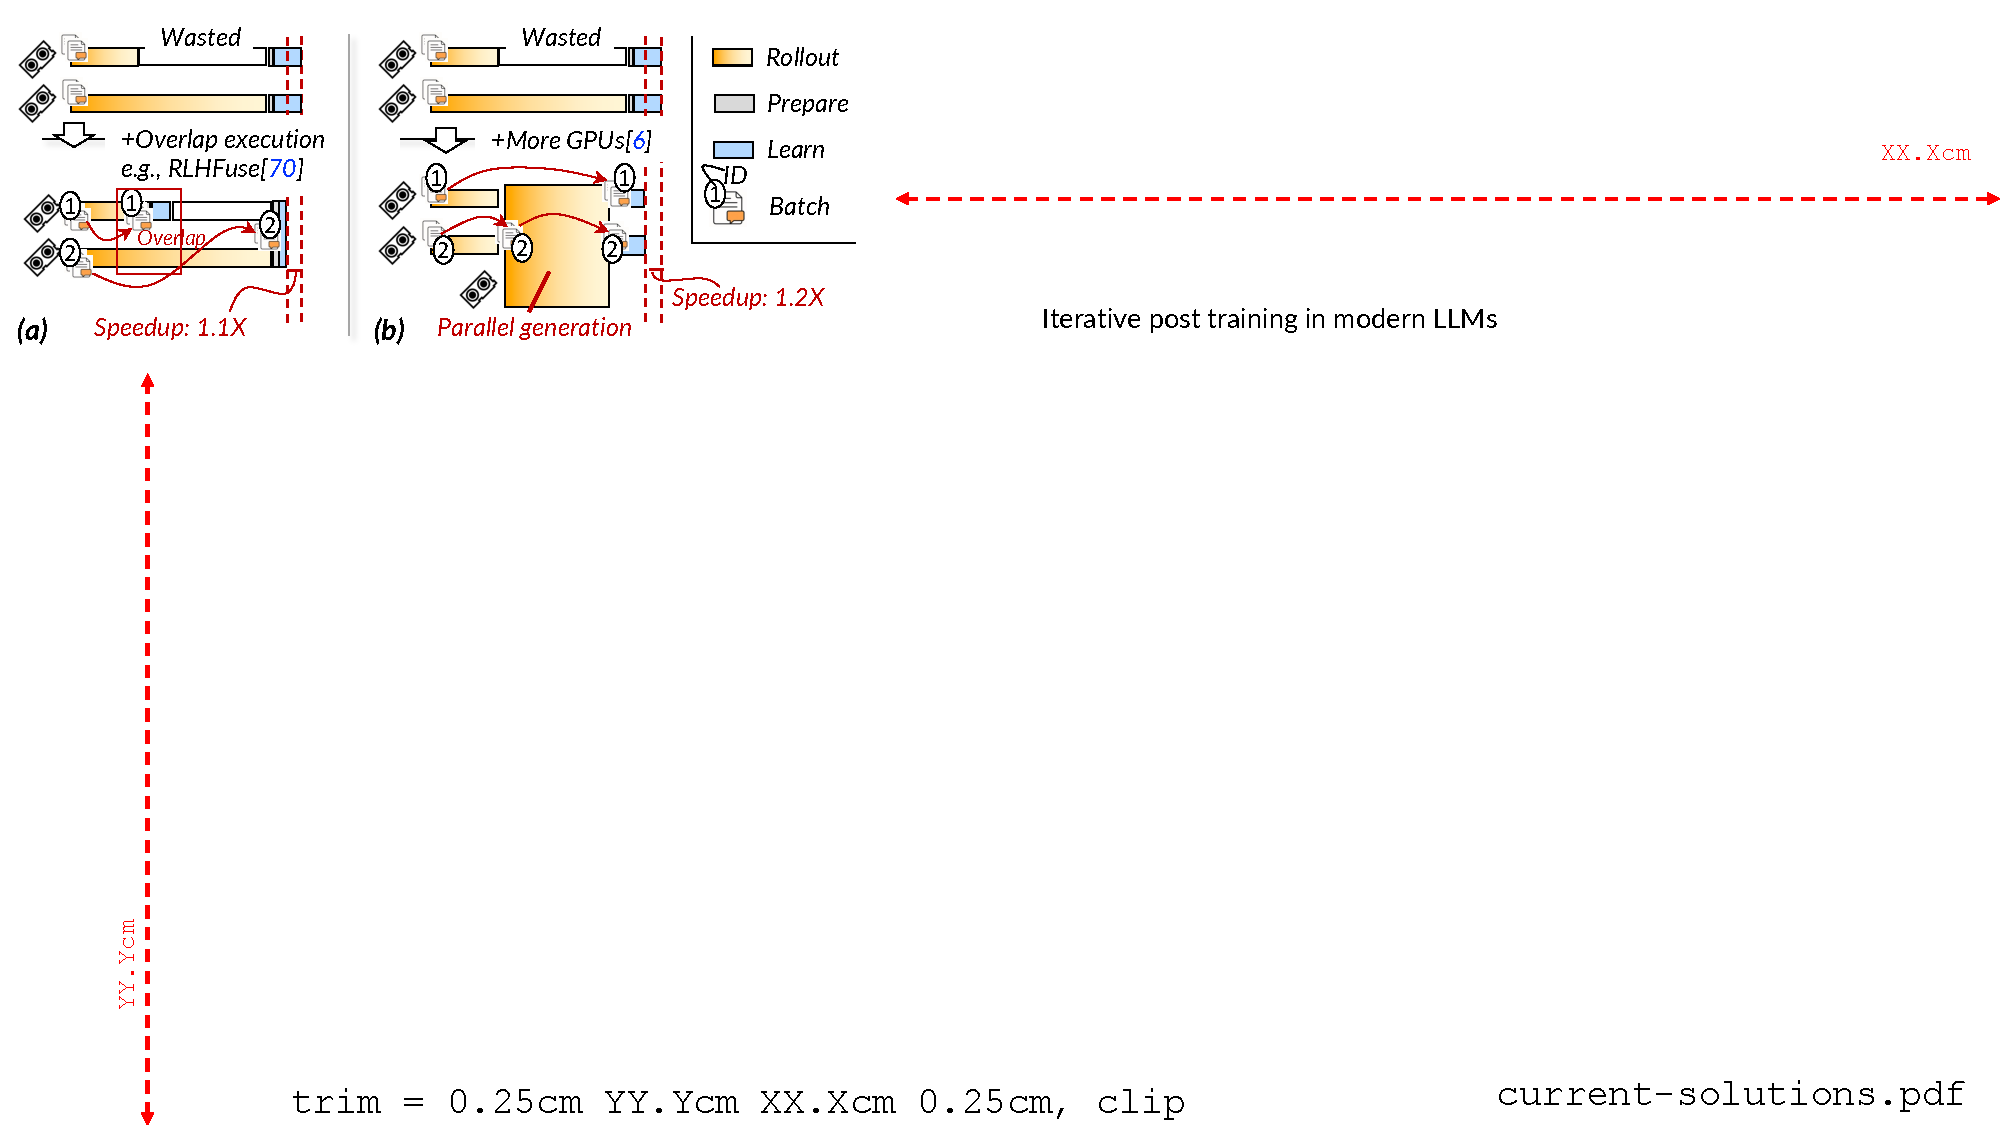
\includegraphics[width=1\linewidth, trim=0.25cm 12.78cm 18.75cm 0.25cm, clip]{figs/current-solutions.pdf} 
        \end{minipage} \\[0pt]
        \begin{minipage}{1\linewidth}
        \caption{\small{%
            (a) An illustration of accelerating post-training via overlapped execution and 
            (b) an illustration of accelerating rollout through scaling to more GPUs.
        }}
        \label{fig:motiv-current-solution}
        \end{minipage} \\[-15pt]
        \end{figure} 


\nospacestitle{Rollout dominates execution time in post-training and suffers significant GPU wastes. \,}
{\fig{fig:data-motivation}} (a) analyzes the contribution of total post-training time in 
typical training tasks:
rollout contributes 70--80\,\% of the total training time.
Since post-training could last for days on hundreds of thousands of GPUs,
accelerating rollout is critical to reducing the overall training cost. 

There exists significant space for improvement for rollout 
because many GPUs are idle during the rollout phase due to the long-generation tail problem.
{\fig{fig:data-motivation}} (a) shows the GPU bubble in long-tailed rollout:
on a {DAPO-32B-20K} trace, we observed averagely {50\,\%} of the total GPU time is wasted
on waiting for the slowest worker to finish.
Rollout time differs significantly across workers
even with the same per-worker batch size,
because the number of tokens required to solve different tasks varies significantly,
and the exact number is hard to predict in advance as they are determined by the LLM outputs.
Moreover, the waste increases as training progresses because as the model becomes "smarter",
it tends to generate more tokens to solve particular tasks~\cite{deepseek-r1}.
%\RX{In comparison, the prepare and learn phases has higher computation efficiency
%and exhibit minimal waste with common training optimizations~\cite{ulysses-sp,DBLP:journals/corr/abs-1909-08053}.}

\stitle{Reducing GPU waste via overlapping achieves a minor speedup for long-tail generation. \,}
An intuitive solution to reduce wasted GPU time is to overlap other phases with the current rollout:
As shown in {\fig{fig:motiv-current-solution} (a)},
representative solutions like RLHFuse~\cite{rlhfuse} utilize the idle workers
to execute the prepare and learn phases of finished batches (e.g., batch \ding{192}),
overlapping these phases from fast workers with the rollout of slower workers.
While such an overlap cannot accelerate the rollout phase, which is bottlenecked by the slowest worker,
it reduces the end-to-end training time
% because the faster workers can proceed part of the prepare 
% and learn phases ahead.
because once the slowest rollout finishes, more GPUs can participate in accelerating
the remaining phases of the slowest batch (e.g., batch \ding{193}).

However, the speedup from overlapping is limited
because the accelerated prepare and learn phases only contribute a small portion of the overall training time (\eg{about 5\% in {\fig{fig:data-motivation}} (a)}).
As a result, RLHFuse only accelerates post-training by {3\,\%} in traces with long response budget,
with GPU time still wasted, as shown in {\fig{fig:data-motivation}} (b).


\stitle{The sequential-generation nature of rollout is the key obstacle for acceleration. \,}
Another intuitive solution is to dynamically add more computation resources to accelerate the long-tailed workers:
as shown in {\fig{fig:motiv-current-solution} (b)},
once a rollout worker finishes its assigned batch (e.g., batch \ding{192}),
it can help accelerate the generation of unfinished batches (e.g., batch \ding{193}) using
parallel LLM generation techniques like sequence parallelism~\cite{loongserve}.
Moreover, current works~\cite{rlboost} aggressively add more GPUs (e.g., by allocating spot instances)
to accelerate the slow rollout workers without waiting for more GPUs to become idle.
In our example, three workers now process the rollout of batch \ding{193}.
Unfortunately, 
as shown in {\fig{fig:data-motivation}} (b), even if we provision 2\,$\times$ GPUs for rollout, 
the end-to-end training time is only improved by {1.2--1.3\,$\times$}.
The limited speedup is rooted in the 
sequential, memory-bound nature of rollout: 
tokens must be generated one-by-one, 
leaving little room for tensor or sequence parallelism~\cite{loongserve} 
due to the extra communication overhead.
Moreover, data and pipeline parallelism can hardly accelerate 
when memory-bound.

\vspace{2.mm}
\noindent \fbox{
\parbox{0.96\linewidth}{
\noindent {Current systems either suffer from limited speedup or adopt lossy acceleration 
methods like off-policy training or truncating tailed generations,
%which are 
%not always acceptable to algorithm designers,
as summarized in \textsection{\ref{sec:related-work}}. 
We seek an algorithm-agnostic system solution for fast rollout. 
}}
}







